\documentclass[12pt,letterpaper]{report}
\usepackage[margin=1in]{geometry}
\usepackage{graphicx}
\usepackage{amsmath}
\usepackage[font=small,labelfont=bf]{caption}
\usepackage[justification=centering]{caption}
\usepackage{tikz}
\usepackage{circuitikz}
\usepackage{siunitx}
\usepackage{float}
\newlength \figwidth
\setlength \figwidth {0.75\linewidth}

\begin{document}

\title{E153 Laboratory Assignment \#10}
\author{Courtney Keeler and Stephen Pinto\\
Harvey Mudd College}
\date{December 18, 2013}
\maketitle

\section*{List of Materials}
\begin{itemize}
	\item Agilent E360A power supply (x3)
	\item Hewlett Packard 33120A Function Generator
	\item Tektronix 2212 Oscilloscope
	\item Pomona 4550B (10X probe)
	\item 2N2222A transistor
	\item 2N3440 transistor
	\item Standard resistors
	\item Standard capacitors
\end{itemize}

\section*{Purpose}
The purpose of this lab is to build the cascode amplifier designed in Design Project \#2 and verify the performance specifications in lab. The final design of the cascode amplifier is shown in Figure~\ref{fig:circuit}
.
\begin{figure}[H]
\centering
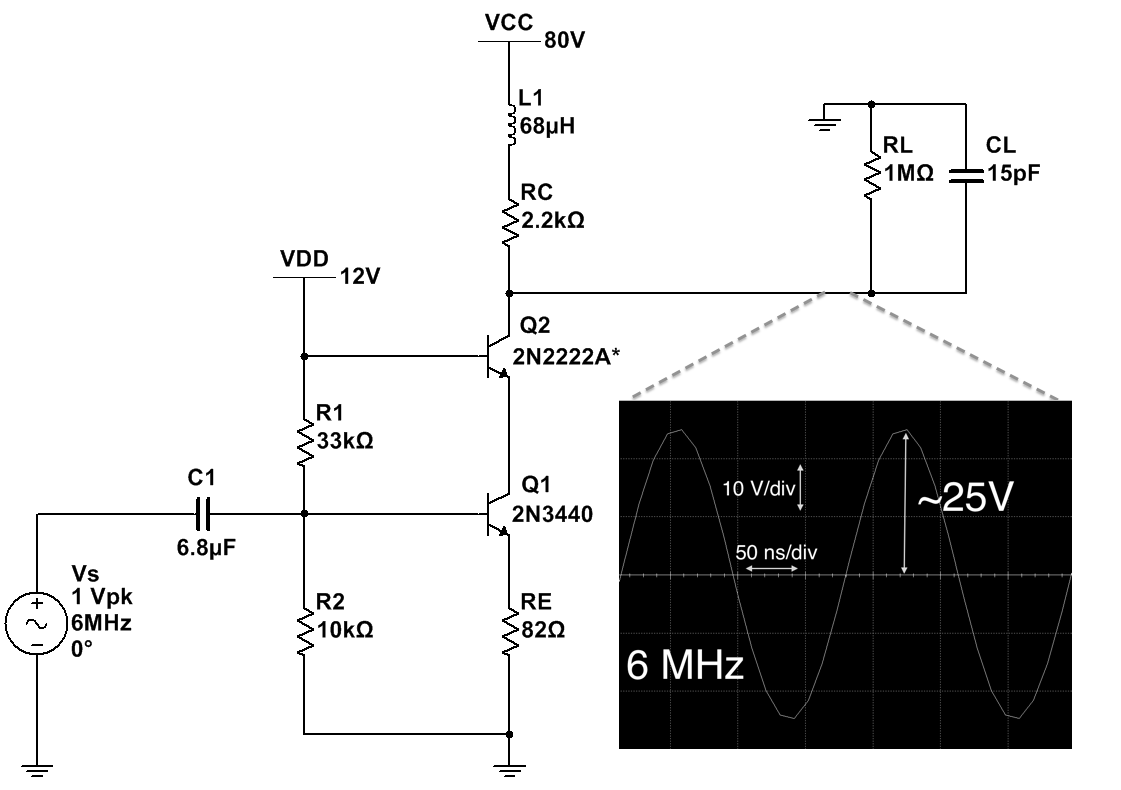
\includegraphics[width=\figwidth, keepaspectratio=true]{lab10_images/result.png}
\caption{High Bandwith Cascode Amplifier designed in Design Exercise 2.}
\label{fig:circuit}
\end{figure}

\section*{Results}

A total of three different DC power supplies supplied the necessary +12V and +80V indicated in the circuit diagram. Two of the power supplies, each set to $\pm 20$V, connected in series to provide the +80 V and the third power supply simply had +12V set to provide the +12V power line. Before constructing the circuit, we measured the component values which are listed in Table!\ref{tab:values}. We could not find a 68 $\mu H$ inductor for $L_1$ or a 6.8 $\mu F$ capacitor for $C_1$ and instead used an 82 $\mu H$ inductor and 10 $\mu F$ capacitor respectively. In the inductor case, a larger inductance will increase the magnitude of the inductive peaking which will push the high cutoff frequency even higher. Similarly, a larger capacitance for $C_1$ will push the low cutoff frequency even lower. Both of these are desireable traits. 

\begin{table}[H]
\centering
\begin{tabular}{|c|c|c|}
	\hline
	 & Designed Value & Measured Value \\
	\hline
	$R_1$ & 33 k$\Omega$ & 32.65 k$\Omega$\\
	\hline
	$R_2$ & 10 k$\Omega$ & 9.88 k$\Omega$ \\
	\hline
	$R_E$ & 82 $\Omega$ & 82.6 $\Omega$ \\
	\hline
	$R_C$ & 2.2 k$\Omega$ & 2.151 k$\Omega$ \\
	\hline
	$C_1$ & 10 $\mu$F & 10.1 $\mu$F \\
	\hline
	$L_1$ & 68 $\mu$H & 82 $\mu$H \\
	\hline
\end{tabular}
\caption{Table of designed versus measured values for the components of the cascode amplifier.}
\label{tab:values}
\end{table}

\subsection*{DC Offset}
With no AC input coming in, the DC offset at the output terminal was 49.06 V. With a target oscillation of $\pm 25$V, a DC offset of about 49 V will make an output signal of 50 $V_{pp}$ oscillate between 24V and 74V. The specifications give a suggested range of 20V to 70V but requires the 50 $V_{pp}$ output for a 2 $V_{pp}$ input. Assuming the gain is correct and that requirement is met (see next section), we think our DC offset is acceptable.

\subsection*{Gain}

\begin{figure}[H]
\centering
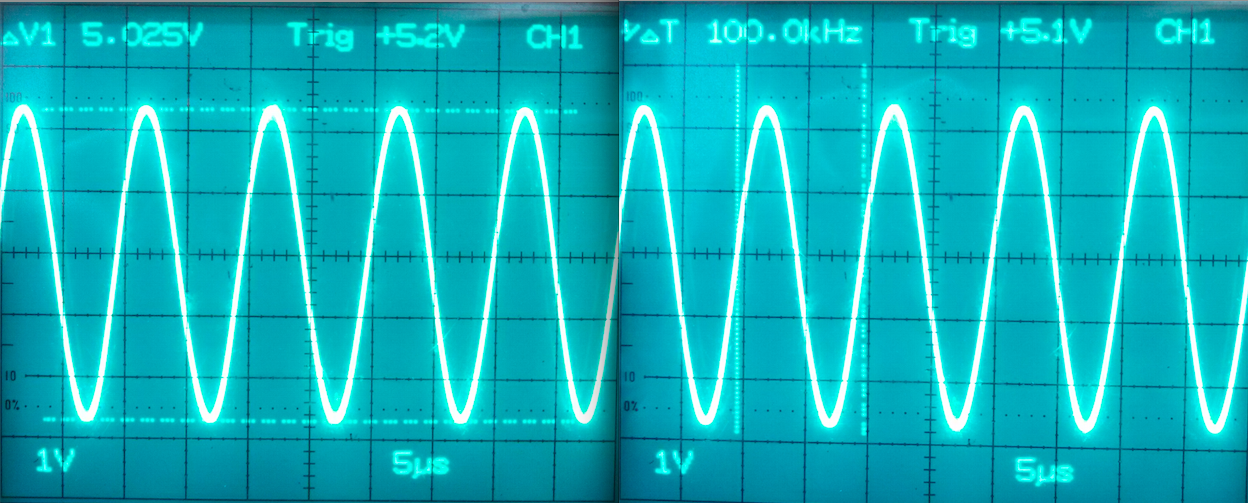
\includegraphics[width=\figwidth, keepaspectratio=true]{lab10_images/100kHz.png}
\caption{Output signal with 2 $V_{pp}$ and 100 kHz input.}
\label{fig:med_freq}
\end{figure}

With an input signal of 100 kHz, well within the bandwidth, and 2 $V_{pp}$, the output signal (shown in figure~\ref{fig:med_freq}) was 50.25 $V_{pp}$, making the gain 25.125. The design specifications ask for a gain of 25. We are satisfied with our 0.5\% difference.

\subsection*{Bandwidth}

\begin{figure}[H]
\centering
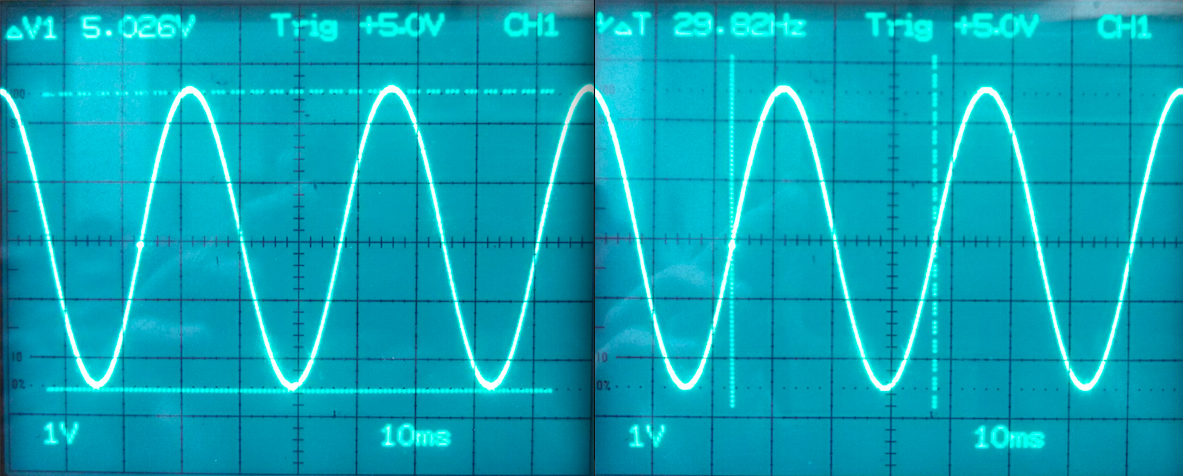
\includegraphics[width=\figwidth, keepaspectratio=true]{lab10_images/low_freq.png}
\caption{Output signal with 2 $V_{pp}$ and 30 Hz input.}
\label{fig:low_freq}
\end{figure}

\begin{figure}[H]
\centering
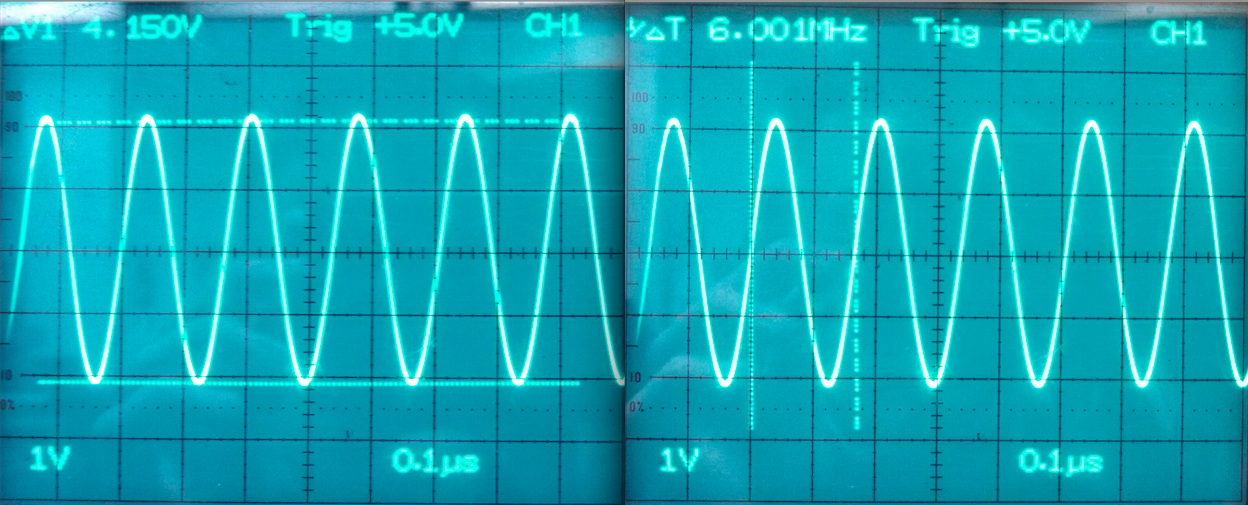
\includegraphics[width=\figwidth, keepaspectratio=true]{lab10_images/high_freq.png}
\caption{Output signal with 2 $V_{pp}$ and 6 MHz input.}
\label{fig:high_freq}
\end{figure}

Figures~\ref{fig:low_freq} and \ref{fig:low_freq} show the output signal with an 2 $V_{pp}$ input signal at 30 Hz and 6 MHz respectively. As can be seen in the figures, the gain for the low frequency input is 25 (as desired) and the gain for the high frequency input is 20.75. Though this is not the desired 25, it is within the 3dB requirent the design specifications list. The actual measured 3dB cutoff frequencies are 3.65 Hz and 6.45 MHz. 

\subsection*{Input Resistance}

The low cutoff frequency is expressed as
$$
f_{c,low} = \frac{1}{2 \pi R_{in} C_1}
$$
$C_1$, listed in table~\ref{tab:values} is 10.1 $\mu F$ and $f_{c,low}$, listed in the bandwidth section, is 3.65 Hz. This makes $R_in$=4.3k$\Omega$, well above the 1k$\Omega$ requirement.

\section*{Conclusion}

In conclusion, this lab has shown that the results achieved in Multisim for this design exercise match reality close enough to not require any tweaks to the circuit. Needless to say, we were pleasantly surprised by these results. As for what we learned by designing a cascode amplifier, refer to our design exercise write up.

\end{document}
